\documentclass{article}
\usepackage[margin=0.7in]{geometry}
\usepackage{amsmath}
\usepackage{amssymb}
\usepackage{bookmark}
\usepackage{graphicx}
\usepackage{float}

\title{Report for Assignment - 2: CS6370 - \\Information Retrieval}
\author{
Harsh Agarwal\\\texttt{CS15BTECH11019}
\and
Sukrut Rao\\\texttt{CS15BTECH11036}
\and
Vishwak Srinivasan\\\texttt{CS15BTECH11043}
}
\date{}

\begin{document}
\maketitle

\section{Introduction}
\begin{flushleft}
    TODO
\end{flushleft}

\section{Task 1: Crawling \& Parsing HTML}
\begin{flushleft}
    TODO
\end{flushleft}
\newpage

\section{Task 2}
\subsection{Text processing of the datasets}
\begin{flushleft}
	Below are the steps for processing:
	\begin{enumerate}
        \item Case Folding - convert all documents to lower case. For example: ``I didn't create Atlantis'' becomes ``i didn't create atlantis''.
        \item Removal of special characters and digits - all special characters (quotes, commas, apostrophes, fullstops, etc.) and digits (0 to 9) were removed. This meant that at the end of this step we had nothing but raw text composed of alphabets alone. For example: ``don't'' becomes ``dont'' and ``ariane-5'' becomes ``ariane''.
		\item Removal of stop words - using \texttt{NLTK}'s corpus of stop words, this was easy.
		\item Stemming - using \texttt{NLTK}'s \texttt{PorterStemmer} we were able to do this.
		\item Lemmatization - for this we used \texttt{NLTK}'s \texttt{WordNetLemmatizer}.
	\end{enumerate}
\end{flushleft}

\section{Plots, Top 20 words and Observations - Chapter Wise}
\subsection{Plots Wise}
\begin{flushleft}
	Below are the frequency distribution plots obtained for 10 out of 62 chapters. 
	\begin{figure}[H]
		\begin{minipage}{0.45\linewidth}
			\centering
			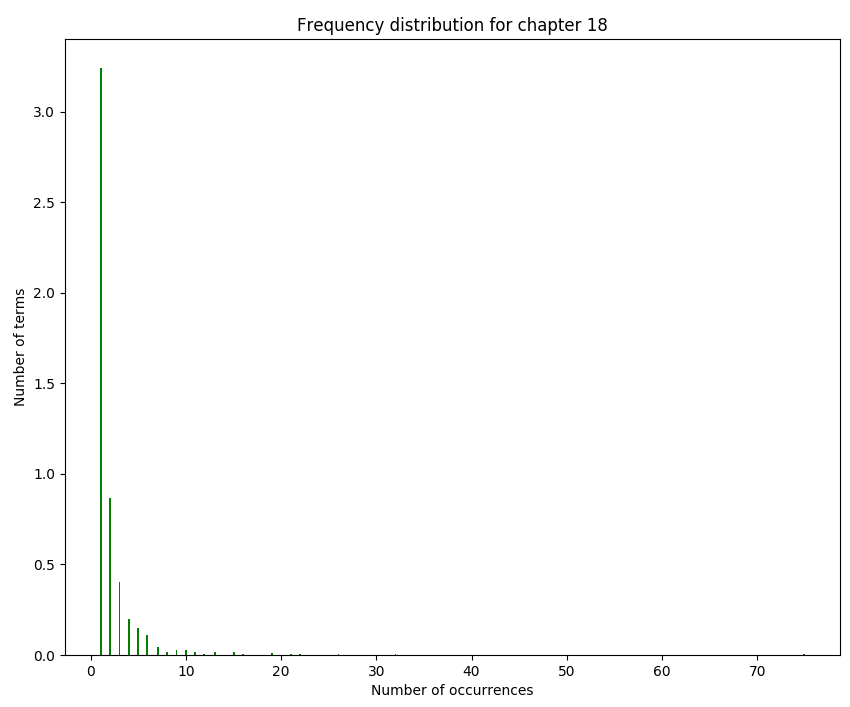
\includegraphics[width=0.75\textwidth]{./images/1-chapter_wise-frequency.png}
			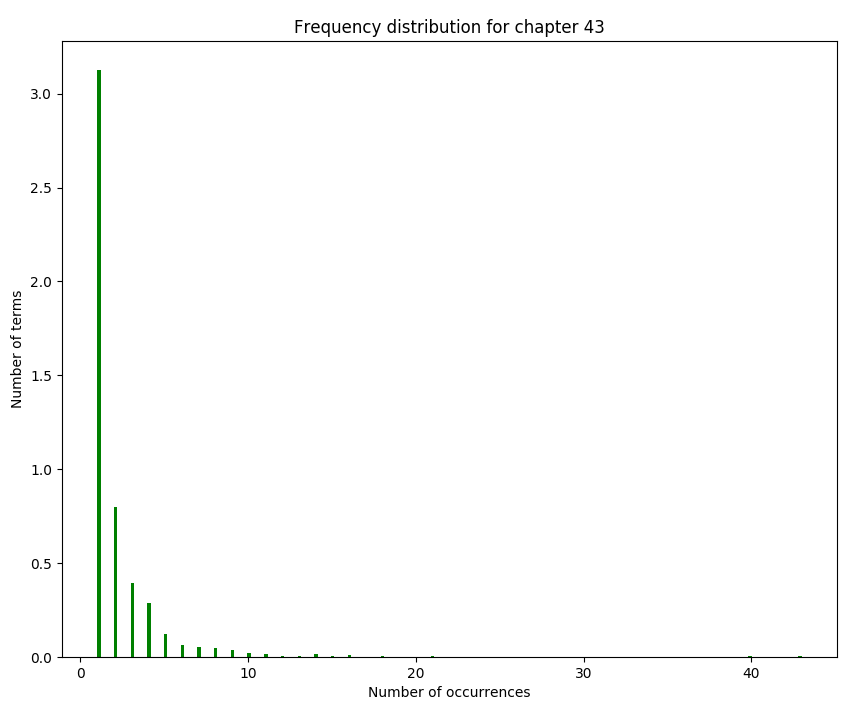
\includegraphics[width=0.75\textwidth]{./images/2-chapter_wise-frequency.png}
			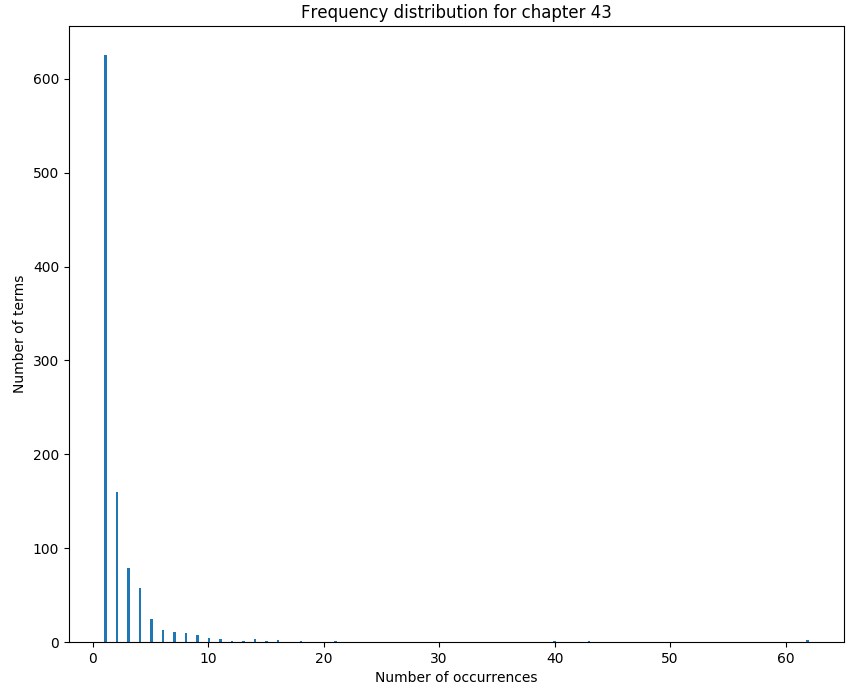
\includegraphics[width=0.75\textwidth]{./images/3-chapter_wise-frequency.png}
			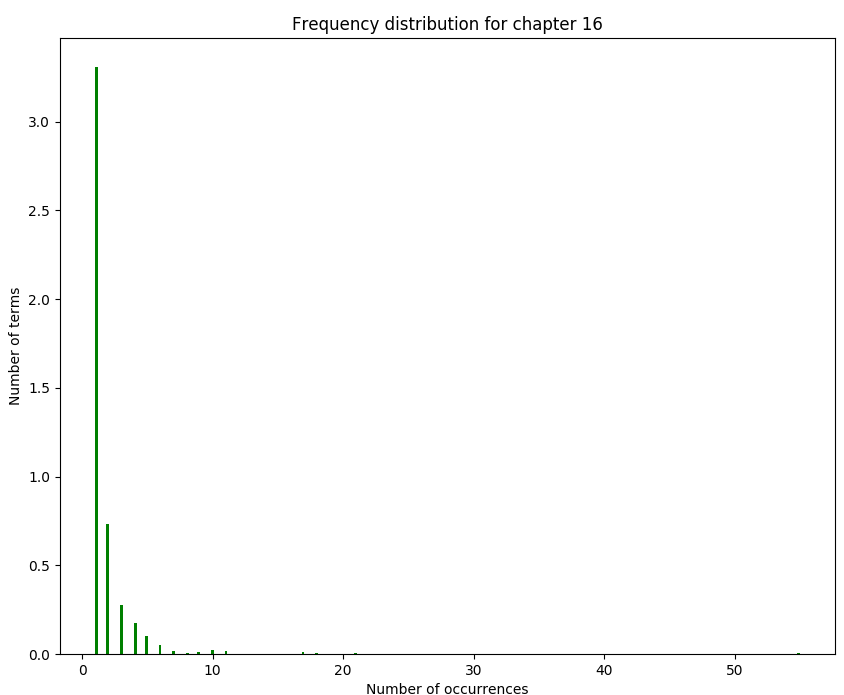
\includegraphics[width=0.75\textwidth]{./images/4-chapter_wise-frequency.png}
			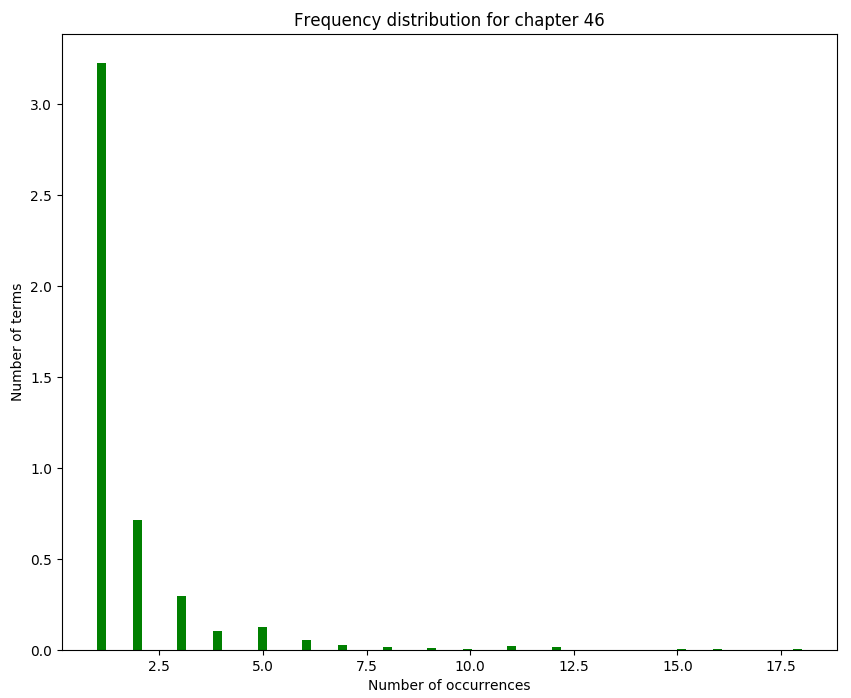
\includegraphics[width=0.75\textwidth]{./images/5-chapter_wise-frequency.png}
		\end{minipage}
		\hfill
		\begin{minipage}{0.45\linewidth}
			\centering
			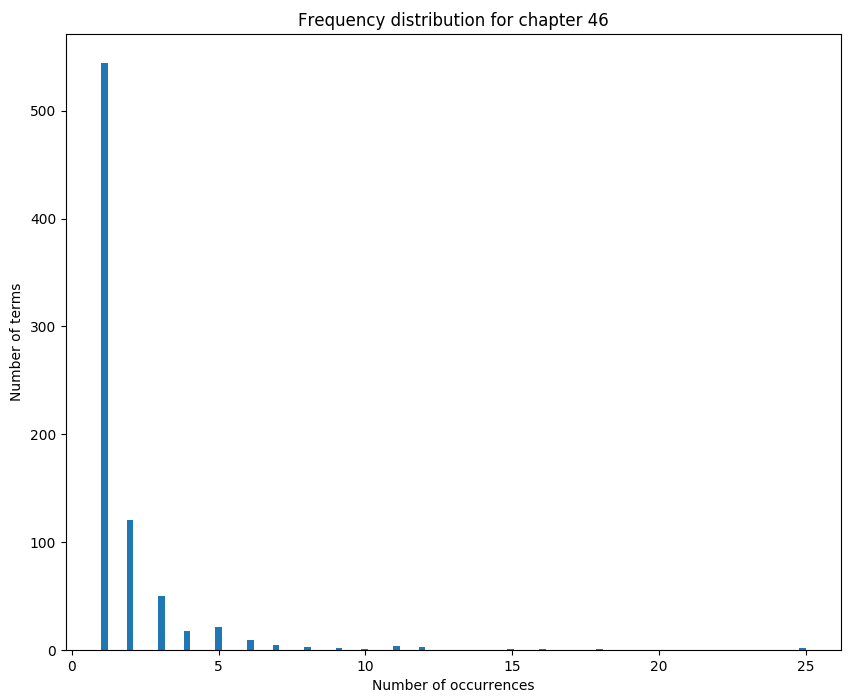
\includegraphics[width=0.75\textwidth]{./images/6-chapter_wise-frequency.png}
			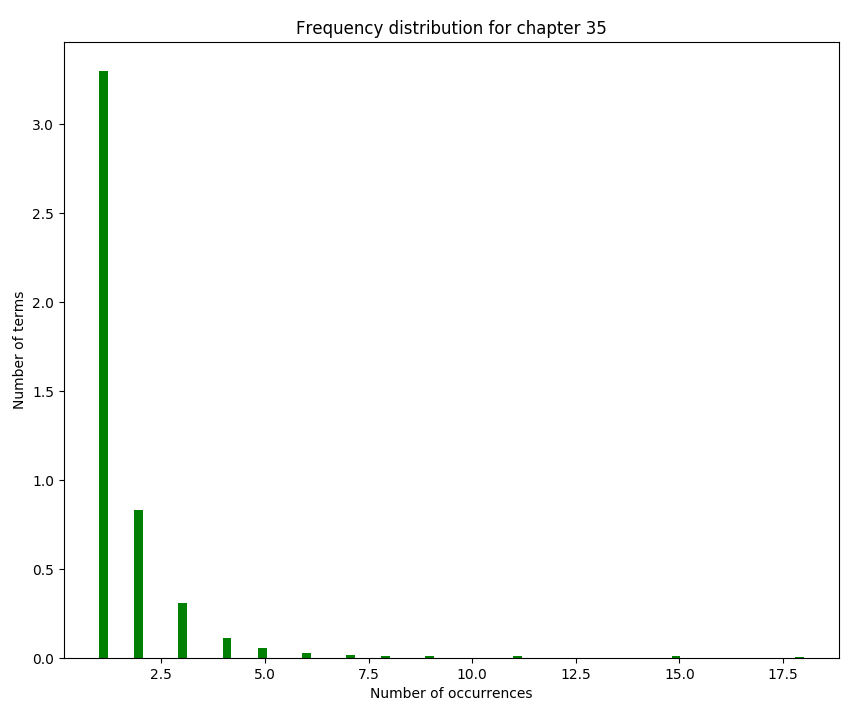
\includegraphics[width=0.75\textwidth]{./images/7-chapter_wise-frequency.png}
			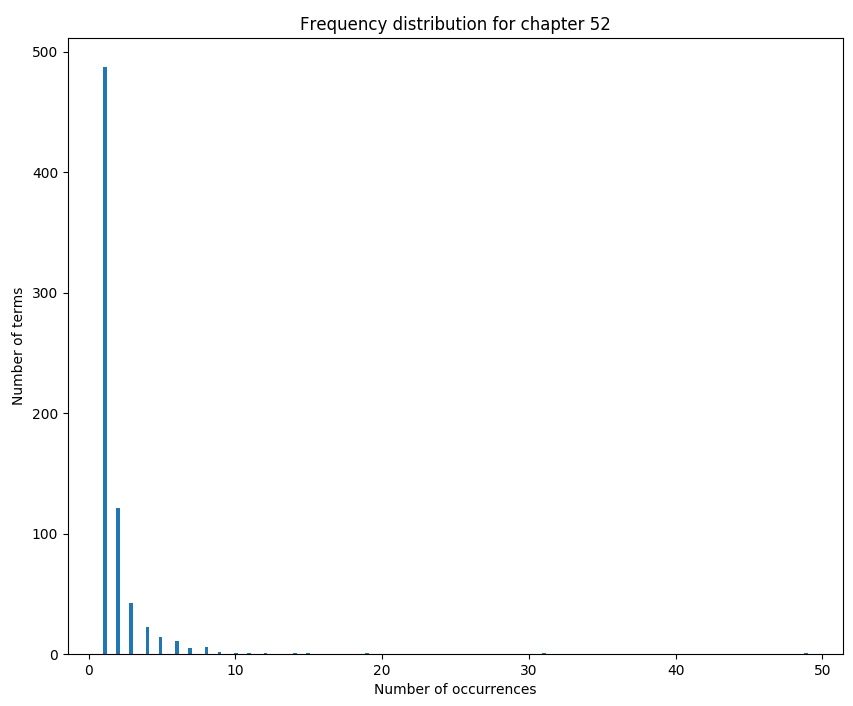
\includegraphics[width=0.75\textwidth]{./images/8-chapter_wise-frequency.png}
			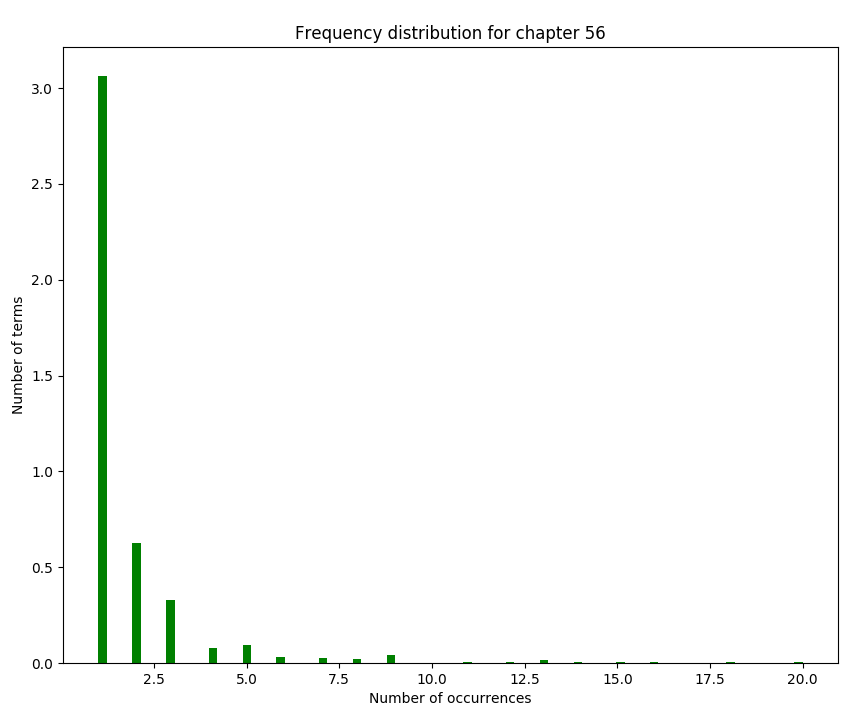
\includegraphics[width=0.75\textwidth]{./images/9-chapter_wise-frequency.png}
			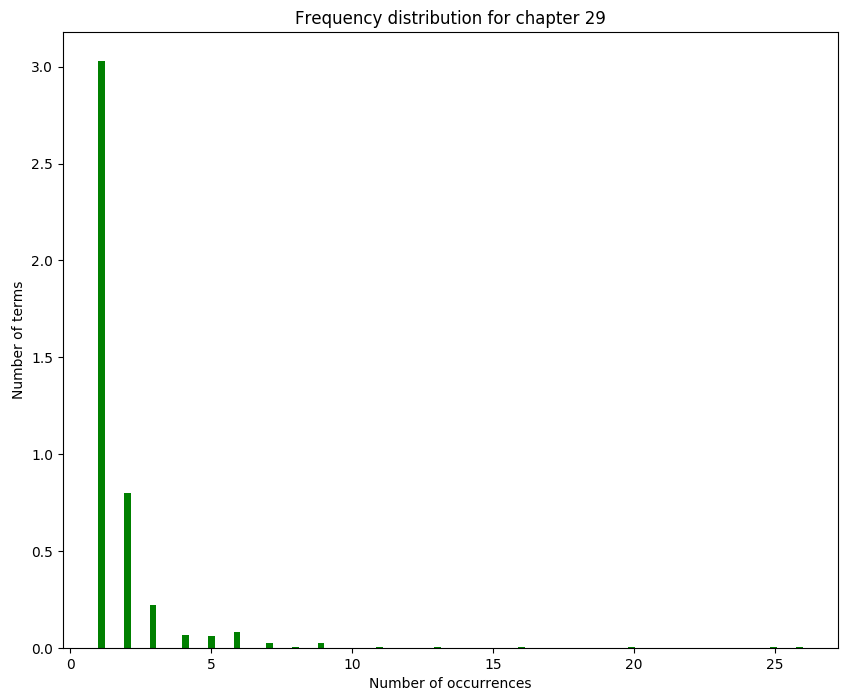
\includegraphics[width=0.75\textwidth]{./images/10-chapter_wise-frequency.png}
		\end{minipage}
		% \caption{Results for Dataset 1 (Left) and Dataset 2 (Right).\newline{}These are log plots for better visualization. Each plot from top to bottom represents a sequence of processing steps.\newline{}These are (ordered from top to bottom): [1, 2], [1, 2, 3], [1, 2, 4], [1, 2, 5], [1, 2, 3, 4, 5]}
	\end{figure}
\end{flushleft}

\subsection{Top 20 words}
\begin{flushleft}
	The top 20 words (based on frequency) obtained for 10 chapters :
	\begin{center}
		\begin{tabular}{|p{0.08\textwidth}|p{0.37\textwidth}||p{0.08\textwidth}|p{0.37\textwidth}|}
			\hline
			Chapter Number & Top 20 Words                                                                                                                     & Chapter Number & Top 20 Words                                                                                                                                  \\
			\hline
			\hline
			62 & \lq\lq, \rq\rq, mr, elizabeth, could, would, said, darcy, bennet, much, must, sister, miss, one, lady, jane, bingley, know, though, never &
			18 & mr, \lq\lq, \rq\rq, darcy, elizabeth, could, said, bingley, though, wickham, sister, say, lady, much, must, may, would, time, collins, dance\\
			\hline
            43 & \lq\lq,\rq\rq, mr, elizabeth, could, gardiner, said, might, master, darcy, thought, much, every, know, room, aunt, time, little, seen, good & 
            47 &  \lq\lq, \rq\rq, could, know, elizabeth, lydia, well, mr, jane, give, think, must, u, would, might, wickham, hope, much, one, colonel  \\
			\hline
			16 & \lq\lq, \rq\rq, mr, darcy, elizabeth, wickham, could, said, lady, man, much, father, pride, manner, collins, phillips, nothing, know, believe, catherine &
			46 & \lq\lq, \rq\rq could, mr, lydia, elizabeth, must, would, letter, though, nothing, one, know, darcy, u, never, first, colonel, well, gardiner\\
			\hline
			53 & \lq\lq, \rq\rq, mr, said, know, could, elizabeth, bingley, bennet, sister, jane, come, see, without, one, soon, must, daughter, looked, never &
			52 & \lq\lq, \rq\rq, would, mr, wickham, could, must, uncle, time, darcy, lydia, sister, know, done, every, much, never, soon, u, though  \\
			\hline
			35 & mr, sister, could, \lq\lq, wickam, father, must, would, last, soon, letter, year, one, feeling, may, shall, every, though, two, friend   &
			56 & \lq\lq, \rq\rq, elizabeth, bennet, lady, miss, catherine, would, mr, ladyship, nephew, shall, must, know, said, say, make, well, mother, family \\
			\hline
		\end{tabular}
	\end{center}
\end{flushleft}

\end{document}


